\documentclass{article}

%% doc settings
\hyphenchar\font=-1 % suppress hyphenation
\setlength\parindent{0pt} % suppress indentation
\usepackage[margin=1.5truein]{geometry} % set page margins


%% core libraries
\usepackage{array}
\usepackage{listings}
\usepackage{fancyhdr}
\usepackage{lastpage}
\usepackage{url}
\usepackage{xcolor}
\usepackage{hyperref}
\usepackage{natbib}
\usepackage{tikz}
\usepackage{tikz-uml}
\usepackage{textcomp}

%% sec libraries
\tikzumlset{fill usecase=white}
\usetikzlibrary{shapes,arrows,positioning,calc}

%% link viz
\hypersetup{
    colorlinks = true,
    linkcolor = red,
    urlcolor = red,
    citecolor = black
}

\tikzset{
    block/.style = {draw, fill=white, rectangle, minimum height=3em, minimum width=3em},
    round/.style = {draw, fill=white, circle},
    tmp/.style  = {coordinate}, 
    sum/.style= {draw, fill=white, circle, node distance=1cm},
    input/.style = {coordinate},
    output/.style= {coordinate},
    pinstyle/.style = {pin edge={to-,thin,black}
    }
}

%% page nums
\pagestyle{fancy}
\fancyhf{}
\fancyfoot[C]{Pg. \thepage \space of \pageref*{LastPage}}
\renewcommand{\headrulewidth}{0pt}

%% begin doc
\begin{document}
\title{SYSEN 6150: Model Based Systems Engineering\\~\\
    \Large Use Case, UCBD, Orig. Req., FFBD
}
\author{
    Nick Kunz [NetID: \url{nhk37}] \hyperlink{nhk37@cornell.edu}{nhk37@cornell.edu}}
\date{September 30, 2022}
\maketitle
\thispagestyle{fancy}

\\~\\
\section*{Use Case Diagram}
The following diagram broadly outlines the reaction from a user of the system and how the system should handle that input.
\\~\\

\begin{tikzpicture}
    \begin{umlsystem}[x=5] {Prediction System} % empty title
        \umlusecase[name=a, y=-1, width=2.5cm] {Accepts}
        \umlusecase[name=b, x=6,width=2.5cm] {Action}
        \umlusecase[name=c, x=6,y=-2,width=2.5cm] {Explain}
        \umlusecase[name=d, y=-3,width=2.5cm] {Rejects}
        \umlusecase[name=e, x=6,y=-4,width=2.5cm] {New Prediction}
    \end{umlsystem}

    \umlactor[y=-2] {User}
    
    \draw (User) -- (a);
    \draw (User) -- (d);

    \draw [tikzuml dependency style] (a) -- node[above] {$\ll \text{extend} \gg$} (b);
    \draw [tikzuml dependency style] (d) -- node[above] {$\ll \text{extend} \gg$} (c);
    \draw [tikzuml dependency style] (d) -- node[above] {$\ll \text{extend} \gg$} (e);
    \draw [tikzuml dependency style] (a) -- node[above] {$\ll \text{extend} \gg$} (c);

\end{tikzpicture}

\newpage
\section*{Use Case Behavioral Diagram (UCBD)}
The following diagram exhibits \textit{one} scenario when a new user begins to use the system.\\

\begin{tabular}{ | m{128pt} | m{128pt}| m{128pt} | }
    \hline
    \multicolumn{3}{|l|}{Prediction System} \\
    \hline
    \multicolumn{3}{|l|}{\textbf{Initial Conditions}} \\
    \hline
    \multicolumn{3}{|l|}{1. The system is in a state on stand by for request.} \\
    \hline
    \textbf{User} & \textbf{System} & \textbf{Outcome} \\ 
    \hline
    The user requests prediction on wait time. & \space & \space \\ 
    \hline
    \space & The system shall respond with estimated wait time. & \space \\ 
    \hline
    The user rejects predicted wait time. & \space & \space \\ 
    \hline
    \space & The system shall respond with explanation for wait time. & \space \\ 
    \hline
    \space & The system shall offer new prediction. & \space \\ 
    \hline
    \space & \space & No direct action is taken by the user. \\ 
    \hline
    \multicolumn{3}{|l|}{\textbf{Ending Conditions}} \\
    \hline
    \multicolumn{3}{|l|}{1. The system is in a state to input user preference for max wait time.} \\
    \hline
    \multicolumn{3}{|l|}{\textbf{Notes}} \\
    \hline
    \multicolumn{3}{|l|}{1. This assumes a new user to the system.} \\
    \hline
\end{tabular}

\\~\\
\section*{Originating Requirements}
The following diagram exhibits a truncated version of the original system requirements.
\\~\\
\begin{tabular}{ | m{28pt} | m{232pt}| m{124pt} | }
  \hline
  \textbf{Index} & \textbf{Originating Requirements} & \textbf{Abstract Function Name} \\ 
  \hline
  \textbf{OR.1} & The system shall not store user PII. &  PII \\ 
  \hline
  \textbf{OR.2} & The system shall input user max wait time. & Max Time \\ 
  \hline
  \textbf{OR.3} & The system shall respond within 3 sec. of request. & Response Time \\ 
  \hline
  \textbf{OR.4} & The system shall not share other user info. & Shared Data \\ 
  \hline
  \textbf{OR.5} & The system shall input local time-zone. & Local Time \\ 
  \hline
  \textbf{OR.6} & The system shall not repeat predictions. & Repeat \\ 
  \hline
  \textbf{OR.7} & The system shall provide one sentence explanations. & Explain \\ 
  \hline
  \textbf{OR.8} & The system shall provide one prediction per request. & Sequence \\ 
  \hline
  \textbf{OR.9} & The system shall terminate at user command. & Terminate \\ 
  \hline
  \textbf{OR.10} & The system shall be accessible offline. & Offline \\ 
  \hline
\end{tabular}

\newpage
\section*{Functional Flow Block Diagram (FFBD)}

The following roughly illustrates the logical flow of information from a subset of the system, as well as where it is coming from and going to.
\\~\\
\textbf{Function 2: Prediction \& Decision Flow as New User}

\centering
\\~\\
%% drawing
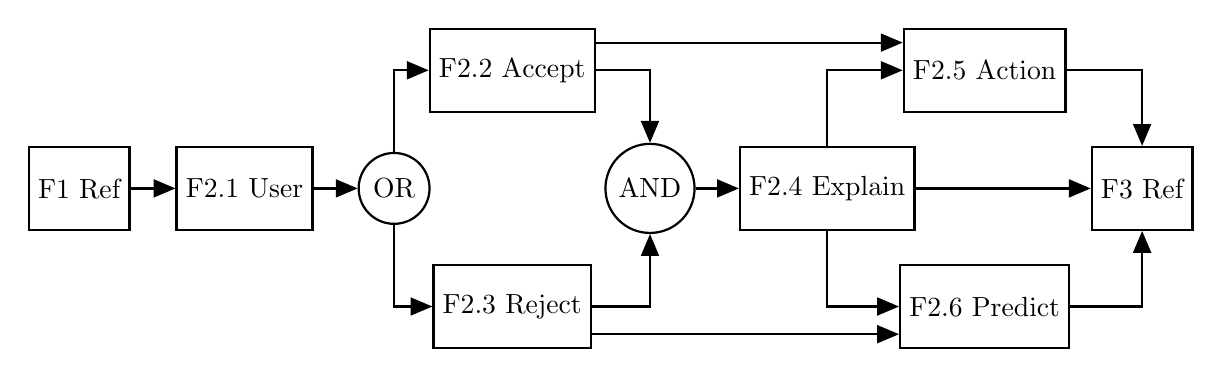
\begin{tikzpicture}[auto, thick, node distance=2cm, >=triangle 45]

    %% func nodes
    \draw node at (-1, 0) [block, name=f1]{F1 Ref};
    \draw node at (1.1, 0) [block, name=f21]{F2.1 User};
    \draw node at (3, 0) [round, name=f22]{OR};
    \draw node at (4.5, 1.5) [block, name=f23]{F2.2 Accept};
    \draw node at (4.5, -1.5) [block, name=f24]{F2.3 Reject};
    \draw node at (6.25, 0) [round, name=f25]{AND};
    \draw node at (8.5, 0) [block, name=f26]{F2.4 Explain};
    \draw node at (10.5, 1.5) [block, name=f27]{F2.5 Action};
    \draw node at (10.5, -1.5) [block, name=f28]{F2.6 Predict};
    \draw node at (12.5, 0) [block, name=f29]{F3 Ref};

    %% flow edges
    \draw[->] (f1) -- (f21);
    \draw[->] (f21) -- (f22);
    \draw[->] (f22) |- (f23);
    \draw[->] (f22) |- (f24);
    \draw[->] (f23) -| (f25);
    \draw[->] (f24) -| (f25);
    \draw[->] (f25) -- (f26);
    \draw[->] (f26) |- (f27);
    \draw[->] (f26) |- (f28);
    \draw[->] (f26) -- (f29);
    \draw[->] (f27) -| (f29);
    \draw[->] (f28) -| (f29);
    \begin{scope}[transform canvas={yshift=10pt}]
        \draw[->] (f23) -- (f27);
    \end{scope}
    \begin{scope}[transform canvas={yshift=-10pt}]
        \draw[->] (f24) -- (f28);
    \end{scope}
\end{tikzpicture}

\end{document}